% \newpage
\subsection{Esercizio 23}
Sia assegnata la seguente perturbazione della funzione $f(x) = sin(\pi x^2)$:
\[
    \tilde{f}(x) = f(x) + 10^{-1} rand(size(x)),
\]
in cui $rand$ è la function built-in di Matlab. Calcolare polinomio di approssimazione ai minimi
quadrati di grado $m$, $p(x)$, sui dati $(x_i, \tilde{f}(x_i))$, $i = 0, \dots, n$, con:
\begin{eqnarray*}
    x_i = i/n, & & n = 10^4.
\end{eqnarray*}
Graficare (in formato $semilogy$) l'errore di approssimazione $\|f - p\|$ (stimato come il massimo
errore sui punti $x_i$), relativo all'intervallo $[0, 1]$, rispetto ad $m$, per $m = 1, 2, \dots, 15$.
Commentare i risultati ottenuti.
\newline \textbf{Soluzione:}

Eseguendo lo script \nameref{cod:23} si ottengono i risultati contenuti nella figura \ref{fig:es22}.
\begin{figure}[!ht]
    \centering
    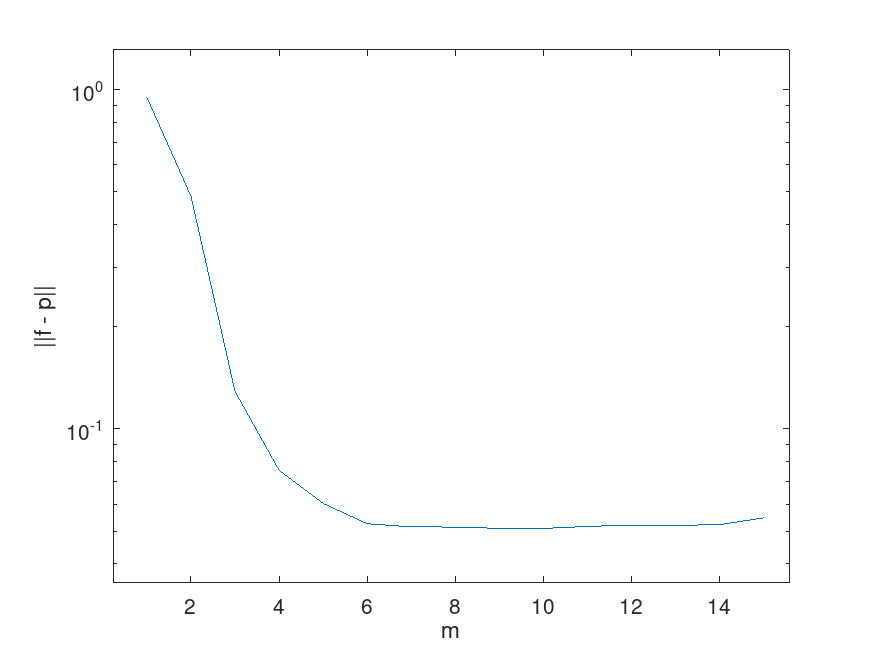
\includegraphics[width=16cm,height=10cm,keepaspectratio]{capitolo5/es23_figure.png}
    \caption{logaritmo di errore}
    \label{fig:es23}
\end{figure}
\FloatBarrier
L'errore decresce molto velocemente inizialmente, ma superato il valore di $m = 5$, si stabilizza
senza azzerarsi.
